\documentclass[12pt]{article}
\usepackage{graphicx} % Required for inserting images
\usepackage{mathtools}
\usepackage{amsmath}
\usepackage{gvv-book}
\usepackage{gvv}
\usepackage[shortlabels]{enumitem}
\usepackage{multicol}

\title{\textbf{7.4.11}}
\author{\textbf{EE25BTECH11004 - Aditya Appana}}
\date{October 1, 2025}
\renewcommand{\labelenumi}{\alph{enumi})}
\begin{document}

\maketitle

\section*{Question}
If the chord $y = mx + 1$ of the circle $x^2 + y^2 = 1$ subtends an angle of measure $45\degree$
at the major segment of the circle then the value of $m$ is
\begin{enumerate}
\begin{multicols}{4}
    \item $2 \pm \sqrt{2}$
    \item $-2 \pm \sqrt{2}$
    \item $-1 \pm \sqrt{2}$
    \item none of these
    
    \end{multicols}
\end{enumerate}

\section*{Solution}

The given line subtends an angle $45\degree$ at the major segment of the circle. Therefore, it will subtend $2\times 45\degree = 90\degree$ at the centre of the circle.\vspace{0.6cm}\\
The line $y = mx + 1$ can be expressed as:
\begin{align}
    \myvec{m\\-1}^T\vec{x} + 1 =0
\end{align}\\
This line always passes through $\myvec{0\\1}$, which lies on the circle $x^2 + y^2 = 1$ (since $0^2 + 1^2 = 1$). Therefore one point of intersection is $\myvec{0\\1}$.\vspace{0.6cm}\\
Let the other point of intersection be $\vec{P}$. $\vec{P}$ will be a $\pm 90\degree$ rotation of $\myvec{0\\1}$ about the origin.\vspace{0.6cm}\\
The rotation matrix is:
\begin{align}
\myvec{\cos\theta & \sin\theta \\ -\sin\theta & \cos\theta}.
\end{align}\\
Therefore:
\begin{align}
\vec{P}= \myvec{0\\1}\myvec{\cos(\pm90\degree) & \sin(\pm90\degree) \\ -\sin(\pm90\degree) & \cos(\pm90\degree)}\\
\vec{P} = \myvec{1\\0} \text{ or } \myvec{-1\\0}
\end{align}
\begin{align}
\text{If } \vec{P} = \myvec{1\\0}, m = \frac{0-1}{1-0} = -1   \\
\text{If } \vec{P} = \myvec{-1\\0}, m = \frac{0-1}{-1-0} = 1 \\
m = \pm1
\end{align}\\
Therefore, \textbf{d)} is the correct answer.

\begin{figure}[H]
    \centering
    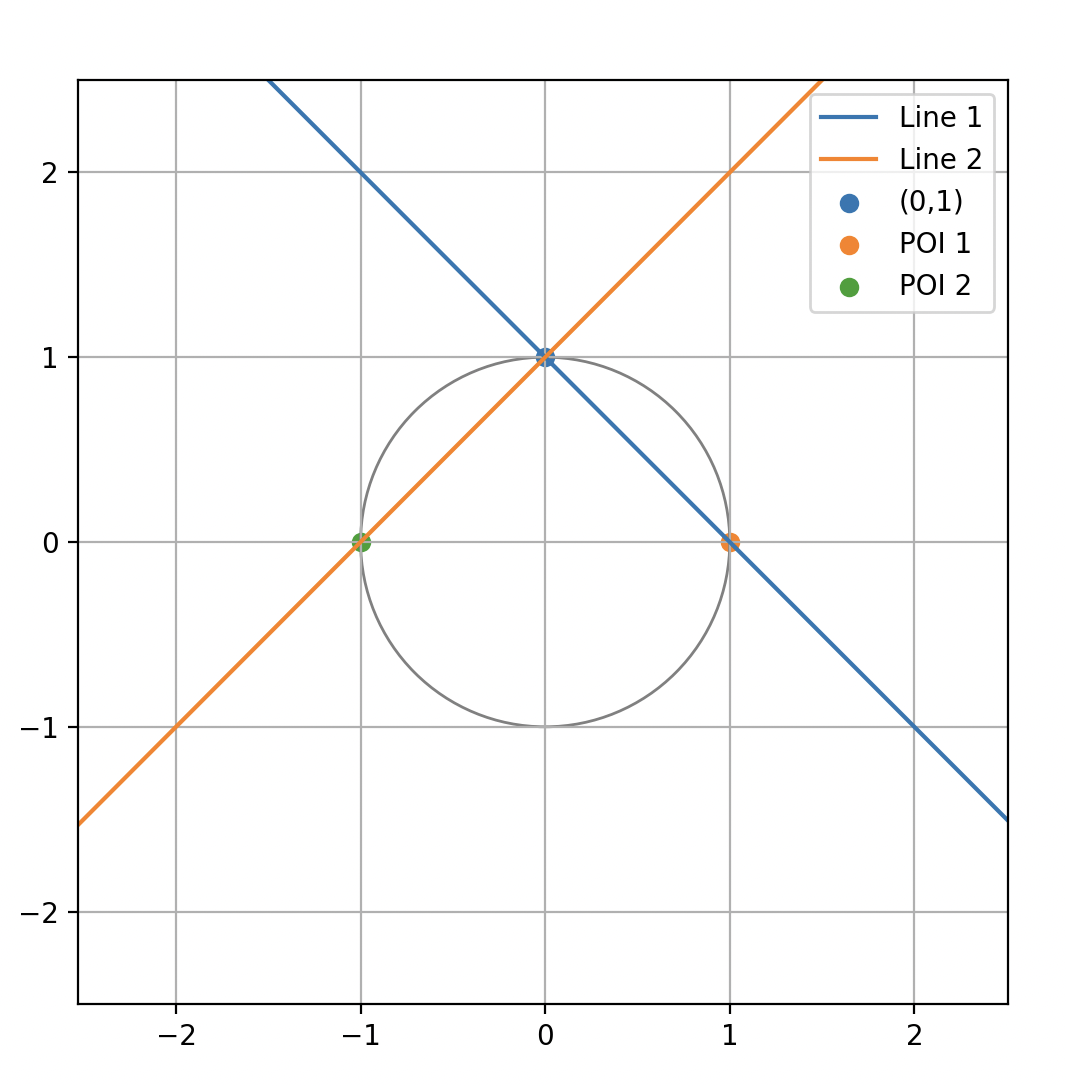
\includegraphics[width=0.6\columnwidth]{Figs/7411.png}
    \caption{Plot}
    \label{fig:placeholder}
\end{figure}




\end{document}